\subsection{Sequence Diagram}

The following two examples are representative of how resources are accessed in our application. The first one shows the login request and the second a generic request that needs authentication.

\begin{center}
    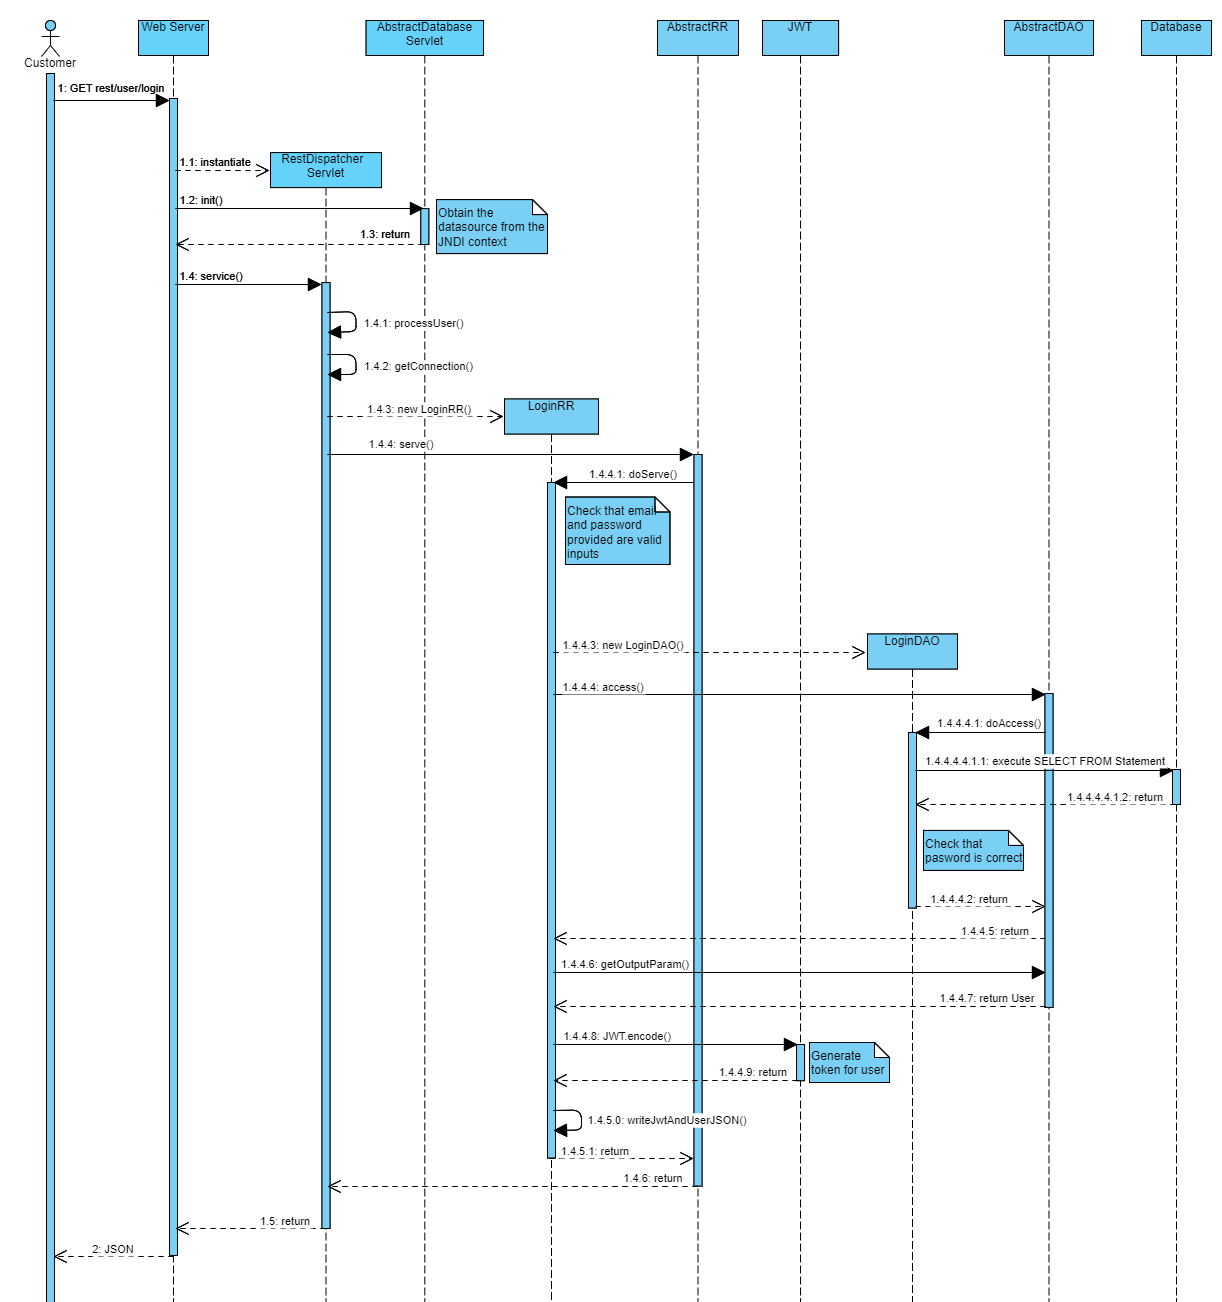
\includegraphics[width=1.0\textwidth]{resources/Sequence-Diagram-Login}
    \captionof{figure}{Sequence diagram for the GET \textit{/rest/user/login} request.}
    \label{fig:sequence-diagram-login}
\end{center}

When a user sends a login request, by performing a GET HTTP request on the \textit{/rest/user/login} URI, the Tomcat web server checks if the URL is mapped to a filter. The login operation doesn't require authentication, therefore the request is forwarded to the RestDispatcher servlet. The dispatcher is tasked with processing the URI and passing the request to the correct RR(REST Resource) class, which is LoginRR in this case. The RR validates the email and password as correctly formed and creates a new DAO(Data Access Object) to retrieve the user registration information from the database. After executing the SELECT FROM statement, the database returns the table row associated with the requested user(if it exists) and the DAO can now check that the password is correct by comparing it with the one in the database. At this point the control returns to LoginRR, that invokes the encode method from the JWT(JSON Web Token) class to extract the token for the user. The JWT and the corresponding User object are encoded in JSON format using the Jackson library and sent back as a response to the user.

\begin{center}
    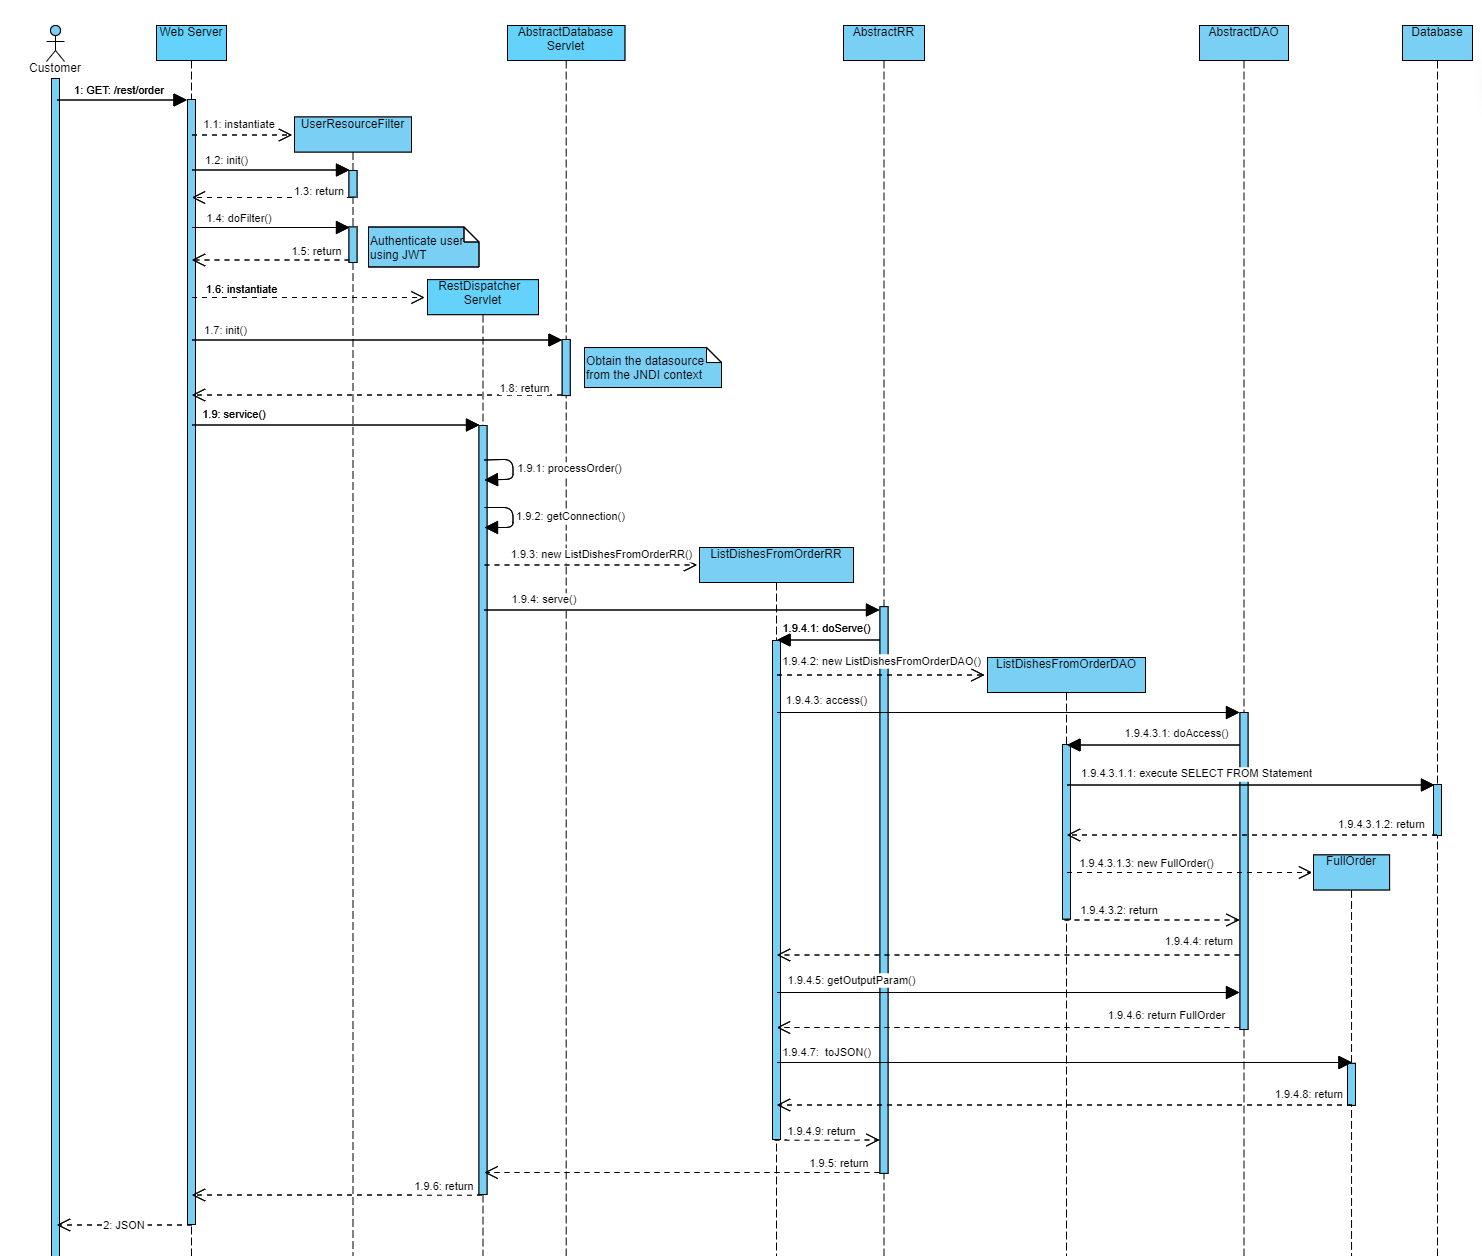
\includegraphics[width=1.0\textwidth]{resources/Sequence-Diagram-List}
    \captionof{figure}{Sequence diagram for the GET \textit{/rest/order} request.}
    \label{fig:sequence-diagram-list}
\end{center}

When a user asks to see the cart information, by performing a GET HTTP request on the \textit{rest/order} URI, the Tomcat web server checks if the URL is mapped to a filter. In this case there is a mapping from \textit{rest/order} to the UserResourceFilter class. The web server calls \textit{init()} on the filter to set up and then \textit{doFilter()} to authenticate the user. If the process goes as intented, the filter sets the attribute \textit{auth\_user} in the HTTP request to the corresponding User object, otherwise it sends an authentication challenge to the user.
At this point the user should be authenticated and the web server proceeds by instantiating the RestDispatcher servlet. The dispatcher is tasked with processing the URI and passing the request to the correct RR(REST Resource) class, which is ListDishesFromOrderRR in this case. The AbstractRR class, from which the ListDishesFromOrderRR class inherits, reads the \textit{auth\_user} attribute of the HTTP request into a protected field, when firstly instantiated. Therefore, the RR class can access it by inheritance and creates a new DAO to retrieve the list of dishes of the cart from the database. After executing the SELECT FROM statement, the database returns the table associated with the requested user's pending order(if it exists) and the DAO can now create a FullOrder object to contain the data of the Order, Order\_Dish, Dish and Restaurant tables after an SQL JOIN operation. At this point the control returns to ListDishesFromOrderRR, that encodes the FullOrder object into a JSON format response. The message is then sent back to the user.
